\begin{figure}[H]
	\centering
	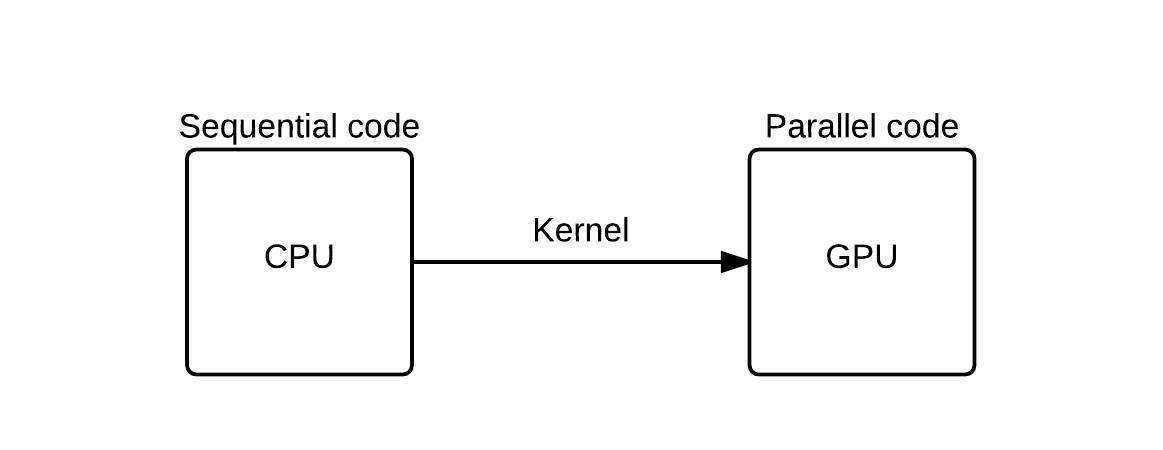
\includegraphics[width=\textwidth]{system_overview/diagrams/programming_model_cpu_gpu.png}
	\caption{Blablabla.}
	\label{programming_model_cpu_gpu}
\end{figure}
Programming for Demolicious will seem familiar for readers with programming experience from technology like CUDA or OpenCL. 
Many applications can be divided into sequential and parallel parts, where each part can benefit from different execution models. \todo{Is this a word<Execution model>?}
On the Demolicious system, the sequential parts of a program will be run by the CPU, and the parallel parts can be performed by the GPU through kernels.
A kernel is a simple program meant to be executed by multiple threads.
The kernels are usually uploaded to the GPU at the start of the program, and then executed when requested by the CPU.
This architecture is well suited for highly parallel tasks such as graphics.
\subsection{Kernels}

\subsection{Memories}

